\chapter*{В}
\addcontentsline{toc}{chapter}{В}

\textbf{Воловня, Воловья, Семинарка} – гора на запад от Детинки, по ней проложен Вознесенский спуск. Название горы указано на планах 1833, 37, 47, 74 годов сначала как Воловня, затем Воловья. Я предполагал, что название происходит не от «вола», а от находившегося выше Пробитого вала, где пробоина была как раз в начале Вознесенского спуска, который проходит этой горой. Проем в Пробитом валу (его видно еще на рисунках Абрахама ван Вестерфельда 1651 года), глядел со стороны нынешней Львовской площади примерно на верх Вознесенского спуска. 

Однако на плане Меленского 1803 года есть, под прописной буквой L, «городская воловня» близ Введенской церкви, а воловня это помещение для содержания волов. 

Гора высится над Кожемяками, а Детинка над Гончарами. 

Итак, овраг Кожемяки лежит на восток от горы Воловни, а Вознесенский яр с Петровской улицей по нему – на запад.

Семинаркой гору называли от находящейся там Духовной семинарии, ныне на ее территории и в ее здании – художественная академия.\\

\medskip

\textbf{Варяжские пещеры}

50°25'53.9"N 30°33'48.2"E

Древнейшие пещеры, примыкают к Лаврским и лежат на юг от них, соединены с Дальними пещерами, расположены под нынешним Спивочем полем, мероприятия на коем не могут благотворно отражаться на состоянии пещер. Закрыты для посетителей.

Согласно сведениям Патерика Печерского, монахи неоднократно раскапывали эти пещеры и находили там «сосуды многоценные», злато и сребро. Закревский цитирует Арсеньевскую рукопись 1406 года, которая уточняет, что сосуды были «латинские»:

\begin{quotation}
В житии св. отца нашего Антония поведается Варажьская поклажа есть, понеже сосуды Латыньскии суть; сего ради Варяжьская пещера зовется и доныне. Злата же и сребра бещисла много.
\end{quotation}

\medskip

\textbf{Васильковская застава} – в 19 веке, застава на левом берегу Лыбеди, около нынешнего Демиевского путепровода, примерно на месте, где ныне часть Океан Плазы, обращенная к Лыбеди. Переезд через реку был именно там, возле впадения в Лыбедь речки Совки.\\

\medskip

\textbf{Васильковские рогатки, Печерские рогатки} – слободка, существовала с 18 по начало 19 века около пересечения нынешних Цитадельной и Московской улиц. Название от Васильковских ворот Старой Печерской крепости, на их месте ныне пятиэтажка по Лейпцигской, 3. 

В слободке поселились прежние жители Печерского городка, снесенного во время строительства крепости. В конце 19 века слободку именовали Печерскими рогатками. Была снесена при строительстве уже Новой Печерской крепости, жители переселены в Новое Строение.

При слободе была деревянная церковь святого Владимира, почти на ее месте\footnote{50°26'01.5"N 30°32'43.2"E} ныне дом по адресу Цитадельная 15/9. Конечно, дом занимает много больше площади.

В конце 18 века слободка именовалась Печерские рогатки.
\\

\medskip
%, остатки коих находятся во дворе дома Цитадельная 15/9.

\textbf{Васильчикова дача}

Занята ныне парком Нивки, была владениями киевского генерал-губернатора Иллариона Васильчикова (1805-1862), где у него был поначалу хутор Васильчики, а потом Александр II еще землицы подкинул. Всего получилось 55 десятин с прудами, пахотными землями, лесом и прочим. Во владениях у семьи Васильчикова стоял двухэтажных особняк.
 
После смерти генерал-губернатора, земля была подарена вдовой Зверинецкому Свято-Троицкому монастырю, а после революции национализирована. 

На территории бывшего хутора Васильчики (50°27'44"N 30°25'15"E), среди живописных яров, на горе над Сырцом с прудами, облюбовали себе место отдыха от трудов партийные боссы, и позже это место прослыло еще одной Дачей Хрущова\footnote{Развалины дома тут – 50°27'43"N 30°25'16"E}. Некоторое время спустя на ее территории был детский кинотеатр. Некоторые местные, в зависимости от поколения, называют здание Дачей Коротченко.

На 2020 год сохранилось полуподземное сооружение, и двухэтажный особняк Дачи, с выбитыми окнами и обрушенными перекрытиями. Внутри всё завалено кирпичами и загажено. Со стороны есть дыра – вход в подвал, он залит водой и там каким-то чудом из крана льется холодная вода, небось десятилетиями.

На восточном берегу пруда\footnote{50°27'49"N 30°25'27"E} к востоку от Дачи есть остатки старинного погреба.\\  
%РАСШИРИТЬ СТАТЬЮ

\medskip

\textbf{Веник} – жилмассив Виноградарь, прежнее урочище Выгода.\\

\medskip

\textbf{Верхнее Лыбедское} – село, упомянуто в генеральном описании Левобережной Украины 1765-69 годов. Там же указано село Нижнее Лыбедское.\\

\medskip

\textbf{Верхний Кудрявец} – слобода, упомянута в генеральном описании Левобережной Украины 1765-69 годов. Там же указан и Нижний Кудрявец, как отдельная слобода.\\

\medskip

\textbf{Веселый майдан}, урочище – местность на юг от перекрестка Салютной и Академика Туполева, по обе стороны от последней улицы и до улицы Эстонской. На 2020 год там юг аэропорта «Святошино», авиационный завод имени Антонова, и строительство огромного ЖК на месте тепличного хозяйства, существовавшего по 2017. 

На север же от перекрестка есть парк «Веселка», названием напоминающий об урочище.\\

\medskip

\textbf{Верхняя Соломенка} – «основная» Соломенка, включает в себя Кучмин яр.\\

\medskip

\textbf{Верхняя Теличка} – южный склон холма ботсада, точнее часть этого склона, лежащая между Караваевщиной и полотном железной дороги у подножия холма. За рельсами на восток, между ними и Днепром, лежала Нижняя Теличка.\\

\medskip

\textbf{Ветряная гора}

50°29'44.7"N 30°26'08.5"E

На карте середины 19 века показана по месту нынешнего переулка Старицкого, где на 2022 год частный сектор теснится застройкой ЖК. Там же, граничила востоком с Мусмановским лесом, что покрывал правый берег Курячего брода.\\

\medskip

\textbf{Ветряные горы} – урочище на северо-восток от Западинки, на середину 20 века ограничивалось с юга исчезнувшей ныне улицей Песчаной и Большой Мостицкой, а с востока – Вышгородской. Сейчас Ветряные горы – название жилмассива примерно в тех краях.\\

\medskip

\textbf{Винницкий парк} – небольшой парк на Соломенке, между улицами Винницкой, Эрнста, Народного Ополчения и Воздухофлотским проспектом. Растут березы и тополя. Есть захоронения 1941 года.\\

\medskip

\textbf{Виноградарь} – район между Ветряными горами и лесом Пущи-водицы. Название произошло от одноименного колхоза, который разводил виноград, а вот сведения о происхождении колхоза очень противоречивы.

В начале 20 века в краях Ветряных гор возникают персидский подданный Исаак Иванович Бекас и некий Абрамов. Городская управа в 1907 году дала Бекасу в аренду на 24 года 16 участков городской земли – 17 десятин – на Ветряных горах. Бекас выращивал там виноград и продавал его, заведя магазин на Владимирской, 46. К 1910 году другие садовники тоже взяли на Ветряных горах участки под разведение винограда. Этому способствовала высотная местность.

После революции, в 1928 году, в Киеве возникает трудовая коммуна «Дом народов востока», около ста человек, состоящая из беженцев всех национальностей – греков, ассирийцев, славян, китайцев, армян, лезгинов и других. Поначалу они обосновываются на Святошине, потом перебираются на Ветряные горы. Коммуна основала колхоз, в итоге переименованный в «Виноградарь». Бекасов был там агрономом, Р.С Майсурадзе – первым главой колхоза, а 16-летняя О.Т. Леончук – звеньевой. После Великой Отечественной ее выбрали главой колхоза.

Непонятно, то ли этот колхоз занимал местность хозяйства Бекаса и расширялся, то ли возник в другом месте неподалеку, ибо судя по всему хозяйство Бекаса продолжилось другим колхозом, «Ветряные горы», а под «Виноградарь» земли выделялись новые, отдельно.\\ 

\medskip

\textbf{Виолина} – ДШС 47, дренажная система в ботсаду, в восточном склоне Зверинецкого холма, вход туда – на склоне южнее Выдубицкого монастыря, почти посередине между ним и нижней частью Выдубицкого озера.\\

\medskip

\textbf{Вира} 

50°24'43"N 30°23'16"E

Пруд на речке Борщаговке, во 2-м микрорайоне Южноборщаговского массива, у пересечения улицы Зодчих и Большой окружной дороги. В водоеме водятся черепахи. Одно из народных названий озера – Вонючка.\\

\medskip

\textbf{Витянские поля} – известное еще в первой половине 20 века урочище и одноименная улица (а также переулок) на Демиевке, лежали между Цымбаловым яром и Вознесенско-Китаевской улицами, примыкая с запада к Ма\-ло-Китаевской. Точное положение я пока не могу определить, скорее всего местность занята постройками где-то на нынешнем проспекте Науки.\\

\medskip

\textbf{Военка} – название ходило, по крайней мере, в конце 1960-х применимо к отрезку улицы Подвысоцкого, примыкающей к воинской части, что находилась южнее больницы. Местные пацаны ходили туда искать гильзы. ВЧ ныне застроена ЖК.\\ 

\medskip

\textbf{Водогон} – или поселок ДВС (Днепровской водной станции), находится в лесу Пущи-Вод\-цы между 57, 58 и 112 лесными кварталами (сама станция – оттуда на юго-восток менее чем в километре). Начал застраиваться в конце 1930-х. К стене соснового леса примыкают улицы с одно-двухэтажными домами, хрущовками, да несколькими панельными домами 1970-х годов. Очень зелено, в палисадниках фруктовые деревья, побелены не только их стволы, но и низы бетонных фонарных столбов.\\

\medskip

\textbf{Водяные ворота} – ворота Печерской крепости, направленные в сторону Наводничей. Показаны на карте 1800 года.\\

\medskip

\textbf{Волейков}

50°28'2"N 30°25'49"E

Бывший хутор Волейков (с 1862 года принадлежал дворянину В. Т. Волейку, а с 1821 княгине К.С. Кудашовой), ныне район по правой стороне речки Сырца. Основа района – улицы улицы Кузьминская, Степана Руданского, Новоукраинская, Танковая – все они возникли до первой половины 20 века. По левому берегу реки Сырца – окрестности улицы Черкасской, Магистральная – это тоже Волейков, а не Дегтяри.

Южная часть Волейкова застроена в 21 веке высотками, вместо частного сектора. Жалкие остатки его сохраняются, по 2017 год, на улице Жамбыла Жабаева, ближе к железной дороге, да на Сикорского в тех же пределах, ближе к Сырцу, вдоль коего и проходят рельсы.\\

\medskip

\textbf{Волчий яр} – по многим  дореволюционным картам, это яр на Нижнеюрковской улице, в коем сейчас находится районная котельная «Лукьяновская» (Нижнеюрковская, 53). 

Однако, по сведениям старожила Александ\-ра Емцова, дом на нынешней Соляной 65 имел в 1911 году адрес Волчий яр 91. 

Из книги местного жителя Ясногурского «Киев былой» 1913 года следует, что улицу Волчий яр переименовали на Саксоновскую, хотя рядом уже была другая Саксоновская. Саксоновскую я вижу на картах по крайней мере с 1894 года, только одну, и никогда не видел на картах улицу Волчий яр. 

В справочнике «Весь Киев» за 1911 год (кстати, мой любимый том из этой серии) встречаем одновременно улицы Волчий яр и Саксоновский яр. При этом Волчий яр – длинная, на много дворов, а Саксонский короткая и на 8 дворов.

Судя по всему, Саксоновской улице, что отображена на картах, соответствует нынешняя Соляная улица, поскольку мы знаем, что на Саксоновской было много дворов, а значит она длинная и по протяженности может совпадать с Соляной.

Я бы мог сделать вывод, что местные продолжали называть улицу Волчий яр Волчьим яром и после переименования, того же придерживался справочник, а на картах ее рисовали официально – Саксоновским яром. И старая Саксоновская тоже где-то существовала, не попадая на карты. 

На плане 1874 года Волчий яр как урочище лежит в районе нынешней улицы Лукьяновской между Чмелёвым яром и Антифеевкой, и может быть отождествлен с Чмелёвым яром.

Однако есть карта 1902 года, где показаны не как улицы, но как урочища, Волчий и Саксонский яры, а также Старая Антифеевская Полянка и Новая полянка. Выводы делайте сами, я не берусь. Добавлю также, что в начале 20 века на улице Волчий яр был трактир «Встреча хороших друзей».

\begin{center}
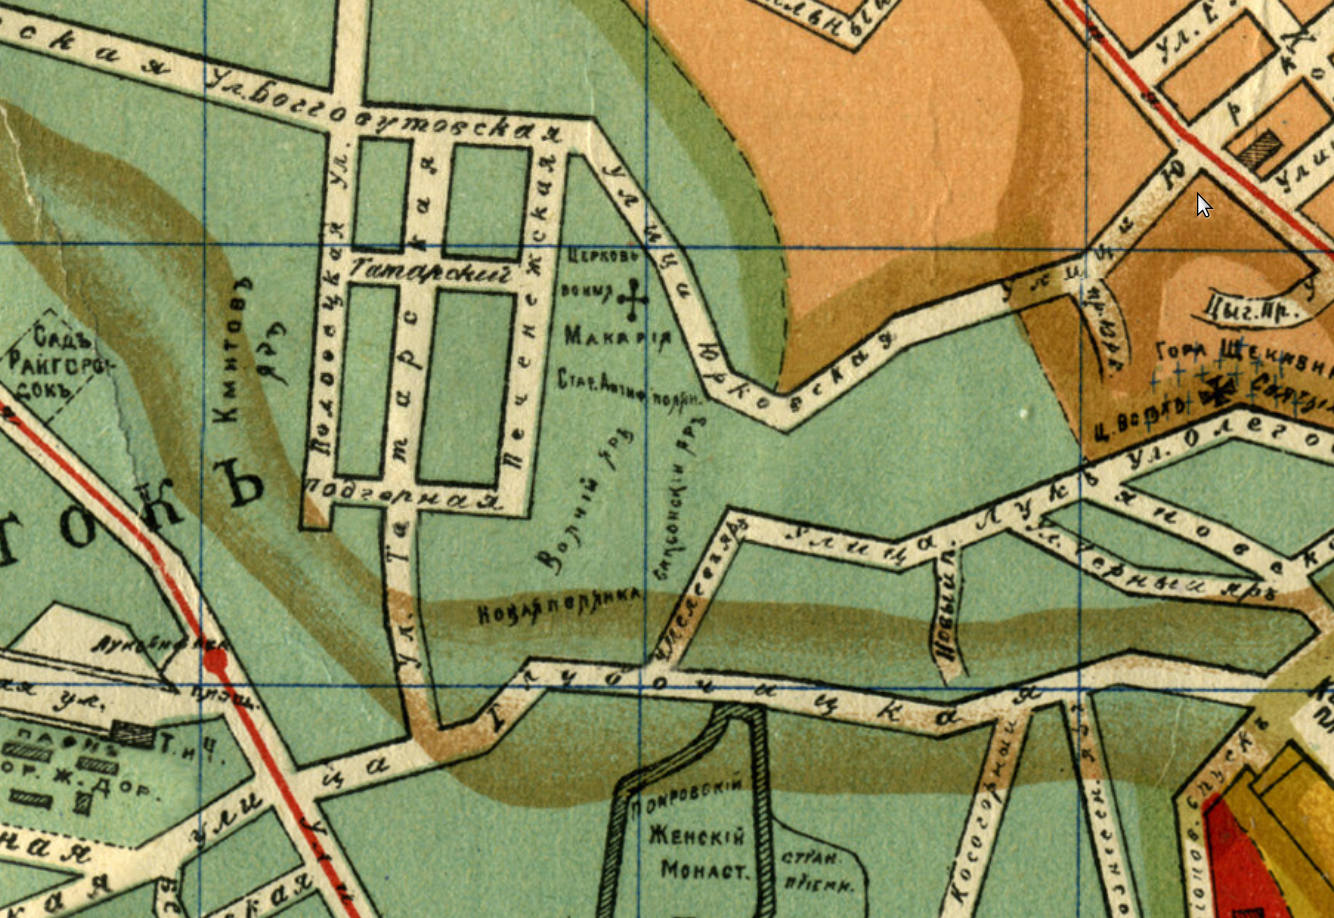
\includegraphics[width=\linewidth]{rpix/volch01.jpg}

\textit{Фрагмент карты 1902 года.}
\end{center}



\medskip

\textbf{Волчий яр} – по крайней мере, в середине 19 века так назывался овраг, в котором протекал ручей, известный ныне как Песочный (приток Лыбеди).

Яр начинался тремя приярками. Один брал начало возле современного северо-западного угла Пушкинского парка, около троллейбусного депо № 2 КП «Киевпасстранс» и дома на Дегтяревской 35/9, где было засыпанное ныне верховье яра.

Другой примерно где детская инфекционная больница на Дегтяревской 25. 

Третий от «дороги на Житомир», его сейчас во многих местах пересекает улица Зоологическая. 

В первом из приярков и начинался ручей Песочный (см. отдельную заметку о нем), но по сводному из трех приярков уже общему яру ручей протекал далее через нынешний Зоопарк и деревню Шулявщину (по месту улиц Шулявской, Ярмолы).\\

\medskip

\textbf{Вовчий яр} – на плане середины 19 века (увы, у меня только кусок его) так подписан «классический» Бабий яр в хорошо известных его пределах. Однако на той же карте, Бабьим яром подписана смежная местность, яр, начинавшийся в конце переулка Чаплыгина и через урочище Граевщину нисходящий к Сырцу в направлении Куренёвского кладбища. Либо, как вариант, яр на карте можно отождествить с улицей Ольжича.\\

\medskip

\textbf{Волчья гора} – возвышенность на Нивках между ул. Щербакова и железной дорогой на север от прудов на речке Сырце в парке Нивки идёт вверх крутой подъём. Улица Эстонская, застроенная частным сектором, прежде именовалась Волчьегорской.

Прежде у Волчьей горы был одноименный хутор, лежащий вдоль Волчьегорского шляха. Улица Эстонская занимает часть последнего.\\

\medskip

\textbf{Вольноживущевка} – окрестности переулка Балакирева на стыке Демиевки и Ширмы, именуется от прежнего названия переулка – переулок Вольноживущих.\\

\medskip

\textbf{Вознесенский яр} – глубокий яр между горой Воловней с ея Вознесенским спуском, и Кудрявцем. Сейчас по яру проходит улица Петровская (ранее Вознесенский яр), а исток яра, на юге, утопает в бурьянах и свалках на склоне, хотя еще в первой половине 20 века улица поднималась и присоединялась к Вознесенскому спуску, там где сейчас храм Василия Великого. 

Яр называется так от улицы, спуска, лежащего по его северному берегу, а спуск (в советское время улица Смирнова-Ласточкина) в свою очередь от Вознесенской церкви, которую в 19 веке снесли и поставили на нее месте либо здание духовной семинарии (ныне Академия искусств), либо южный корпус больницы Академии уже наук.

На южном берегу яра, по улице Кудрявской, над обрывом стоит дореволюционный дом номер 47, о трех этажах, причем с улицы видны только два и они обложены с фасада кирпичом, а вот если глядеть из яра, то дом трехэтажный и с той стороны два верхних обшиты темными от времени досками и дом кажется деревянным.

Берега яра – из суглинка, очень крутые, местами почти отвесные. На дне расположены автобаза и подобные объекты, а одной из террас, возле котельной – кинологический центр, откуда слышен хорош поставленный лай очень солидных, как оперные певцы, собак.\\

\medskip

\textbf{Выгода} – урочище, где на Виноградаре лежит озеро Синее. На стыке 19-20 веков соседствовало востоком с сыпучими песками. На плане 1923 года, Выгода протянулась нижней половиной вдоль урочища Сукачев яр, а верхней вдоль урочища Ветряные горы. И яр, и горы – к востоку от Выгоды.\\ 

\medskip

\textbf{Выдубичи} – древнее урочище, овраг в котором лежит Выдубицкий монастырь. С ним связано предание, что тут «выдыбнул» – прибился к берегу – свергнутый Владимиром с горы у Боричева языческий идол (не Перун, Перун поплыл к Днепровским порогам). Подробнее см. «Ересь о Киеве».

А вот метро «Выдубичи» названо так непонятно почему, ибо лежит между Бусовой и Лысой горами много южнее Выдубичей.\\

\medskip

\textbf{Высшая Лыбедь} – из справочника 1884 года: «сенокос площадью 24 десятины, на реке Лыбедь, у плотины при выезде от предместья Демиевки в город. Прежде здесь был Лыбедский пруд».

Из книги Похилевича «Монастыри и церкви Киева» 1865 года, владение Лавры, дававшее доход 270 рублей:

\begin{quotation}
\noindent Высшая-Лыбедь, бывший пруд с мельницею на Васильковской почтовой дороге. Плотина разорванная от грозового дождя в 1839 году, не возобновлена к поводу разногласия о том, кто должен содержать плотину, чрез которую проходит большой тракт. Ныне на месте пруда заведены огороды, пространством в 23 десятины, отдаваемые в аренду\footnote{Будущие Берлизовы огороды?}. 
\end{quotation}

\medskip

\textbf{Вумовский лес}

50°25'58.0"N 30°21'11.0"E

Лес со старыми могучими соснами и оврагом, в Петропавловской Борщаговке, в нем частично находится парк «Петропавловская Борщаговка». Лес расположен между частным сектором (что на берегу речки Борщовки) и промзоной. В лесу есть родник, выведенный трубой в озеро. На начало 21 века площадь леса составляла 13,4 га, с тех пор местность «осваивается» застройкой, на 2020 год осталось меньше половины.

Название происходит от ВУМ – Киевский завод Вычислительных и Управляющих машин, иначе говоря Электронмаш, который имеет адрес Окружная 4 и соседствует с лесом.\\

\medskip

\textbf{Высокое}

Урочище на Приорке, на плане середины 19 века обозначенное по координатам:

50°30'02.1"N 30°26'45.6"E

То есть к югу от Покровской церкви на Мостицкой улице. Церковь стоит на горбе, потом еще на северо-запад от церкви холм еще повышается, быть может название урочища относилось ко всей этой местности.  На той высокой части холма было прежде кладбище, а теперь небольшой парк с дубом на эдаком кургане. Остатки кладбища сохранились по другую сторону от церкви, да и между церковью и домом Мостицкая, 26 есть террасы\footnote{Кладбище сие было снесено в 1987 году.}.

А ниже церкви в то время стоял, на перекрестке, питейный дом – небось, чтобы нищие, получив под церковью милостыню, несли и пропивали там копеечку.\\

\medskip

\textbf{Вычовка} – см. Совка.\\